 % est et une illustration par la création d'un fichier de configuration de Cooja est présenté dans en annexe~\ref{code:templating}.

L'annexe~\ref{code:deploiement} montre comment de tels procédés peuvent être réalisés à l'aide de l'outil \texttt{fabric}~\cite{fabric}.

Une présentation de l'outil \texttt{fabric} permettant une récupération des logs est proposé dans l'annexe~\ref{code:deploiement}.

L'annexe~\ref{code:parsing} illustre ces traitements par d'une trace \ac{PCAP} vers un fichier \ac{CSV}.

L'annexe~\ref{code:analyse} illustre ces fonctionnalités utilisées par Makesense pour fournir des résultats. 

Dans cette thèse, l'outil utilisé pour obtenir l'intégration continue est Travis-CI, l'annexe~\ref{code:ci} contient un exemple de fichier de configuration typique pour ce service.


% \begin{figure}[ht]
%   \centering
%   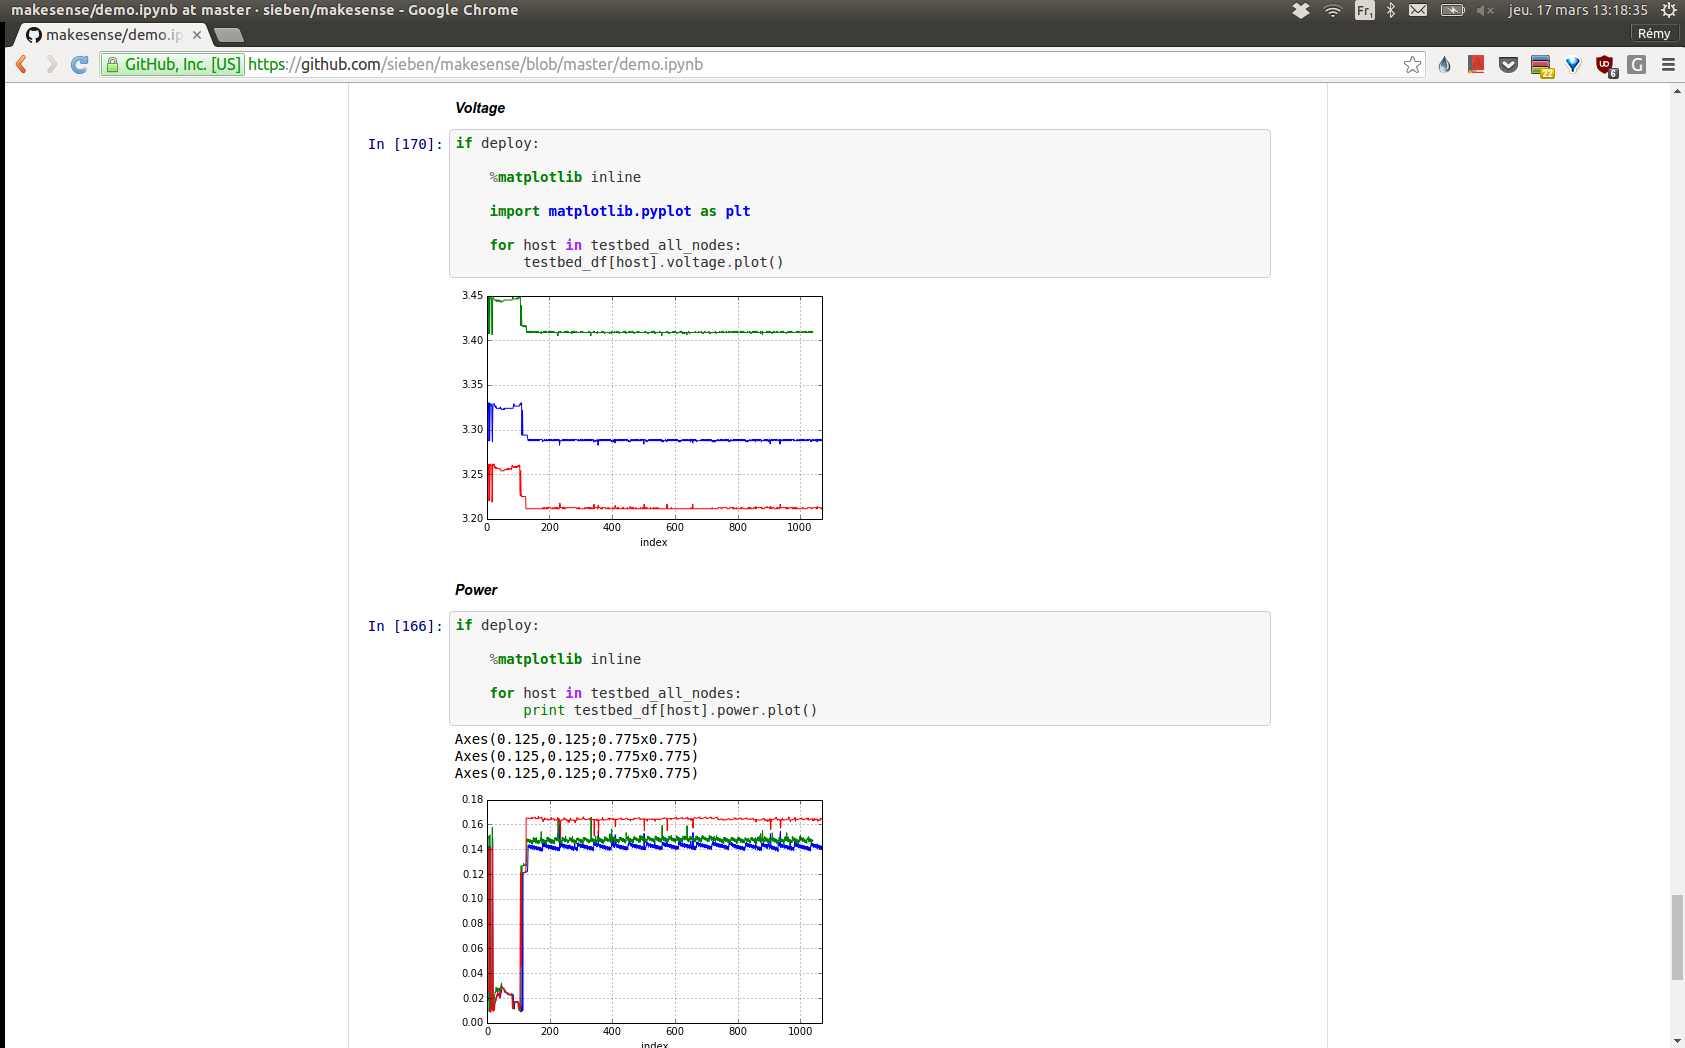
\includegraphics[width=.8\textwidth]{img/jupyter_screenshot.png}
%   \caption{Rendu en ligne d'un notebook hébergé par Github}
%   \label{makesense:fig:screenshot}
% \end{figure}


% \paragraph{Communauté importante}

% Disposer d'une communauté importante est essentiel pour garantir qu'un projet est maintenu et répandu dans de multiples communautés.
% De plus, disposer d'une communauté large permet au débutant de facilement trouver de la documentation et des didacticiels pour gagner en compétence alors que des outils à la diffusion plus restreinte ne peuvent pas assurer un support gratuit avec autant d'efficacité.

% Afin de rester aussi prêt que possible de ses utilisateurs, le projet Jupyter est diffusé sous licence libre et adopte un modèle de fonctionnement ouvert et collaboratif où chacun peut contribuer.
% Cette communauté permet de faciliter les collaborations, l'interopérabilité des solutions et le développement de Jupyter.
% En outre, une large communauté permet de disposer d'un large corpus de documentation et de didacticiels qui sont utiles pour les utilisateurs débutants~\cite{mckinney2012python}.

% % Un autre avantage provenant de l'utilisation d'un format ouvert et spécifié est la constitution d'un écosystème de solutions alternatives pour visualiser un notebook et apporter de nouvelles fonctionnalités avec des logiciels tels que PyCharm, SageMathCloud ou bien encore Beaker Notebook.
% % Ainsi les utilisateurs peuvent utiliser des outils différents et conserver leurs préférences de développement.


% Documenter une expérience est un premier pas nécessaire pour permettre à un humain de tenter de la reproduire.
% L'automatisation d'une expérience poursuit cette démarche en garantissant qu'une machine peut la reproduire.

% En outre, un notebook seul n'est pas utilisable directement, il doit être lancé dans une plateforme adaptée ou bien rendu vers un fichier fixe afin de pouvoir être lu.
% Ainsi afin d'augmenter la diffusion et l'utilisation d'un notebook il peut être commode de disposer d'outils installables ou de services en ligne permettant de dynamiquement rendre et exporter un notebook.

% De plus des solutions existent pour héberger ces notebook dans un espace collaboratif et hébergé~\cite{saravanan2014creating}.
% Ainsi il devient possible d'éditer collaborativement un notebook depuis un simple navigateur web, d'exécuter les cellules de code et cela sans installer de dépendances particulières.

% Actuellement, Contiki~\cite{dunkels2004contiki} est considéré comme le système d'exploitation de référence pour les nœuds capteurs en raison de son implémentation de tous les protocoles exposés au cours du chapitre~\ref{gw}.
% De plus, il est intégré avec le simulateur Cooja~\cite{cooja} qui est combiné avec l'émulateur MSPSIM~\cite{eriksson2007mspsim} afin de simuler le réseau et émuler le fonctionnement des nœuds sur plateforme MSP430~\cite{davies2008msp430}.
% Au cours d'une simulation, le simulateur modélise les interactions dans le réseau via différents modèles de propagation et produit de multiples traces qui enregistrent le comportement des nœuds.
